\section{Digitisation}
\label{sec:digi}

The digitisation procedure is aimed at converting Geant4 SimHits into
reconstructed hits, i.e. reproducing what the electronics of the real
detector will do given an analogue signal, with a signal and a noise
component, passed through analogue-to-digital (ADC) convertors, with a
zero-suppression threshold applied to reduce the data volume, and
finally the calibration back to an energy.

Minimum ionising particles (MIPs) will deposit energy according to a
Landau distribution, whose maximum probable value can be used to
convert Geant4 energies into other relevant quantities. 

\subsection{The MIP signal}

The energy deposited by 50 GeV muons per $2.5\times 2.5$ mm$^2$ cells
is shown in figure~\ref{fig:muHits}. On the left the number of cells
with energy deposits are shown as a function of the layer, and on the
right the energy deposits for layers which have one and only one hit.

\begin{figure}[h!]
  \begin{center}
    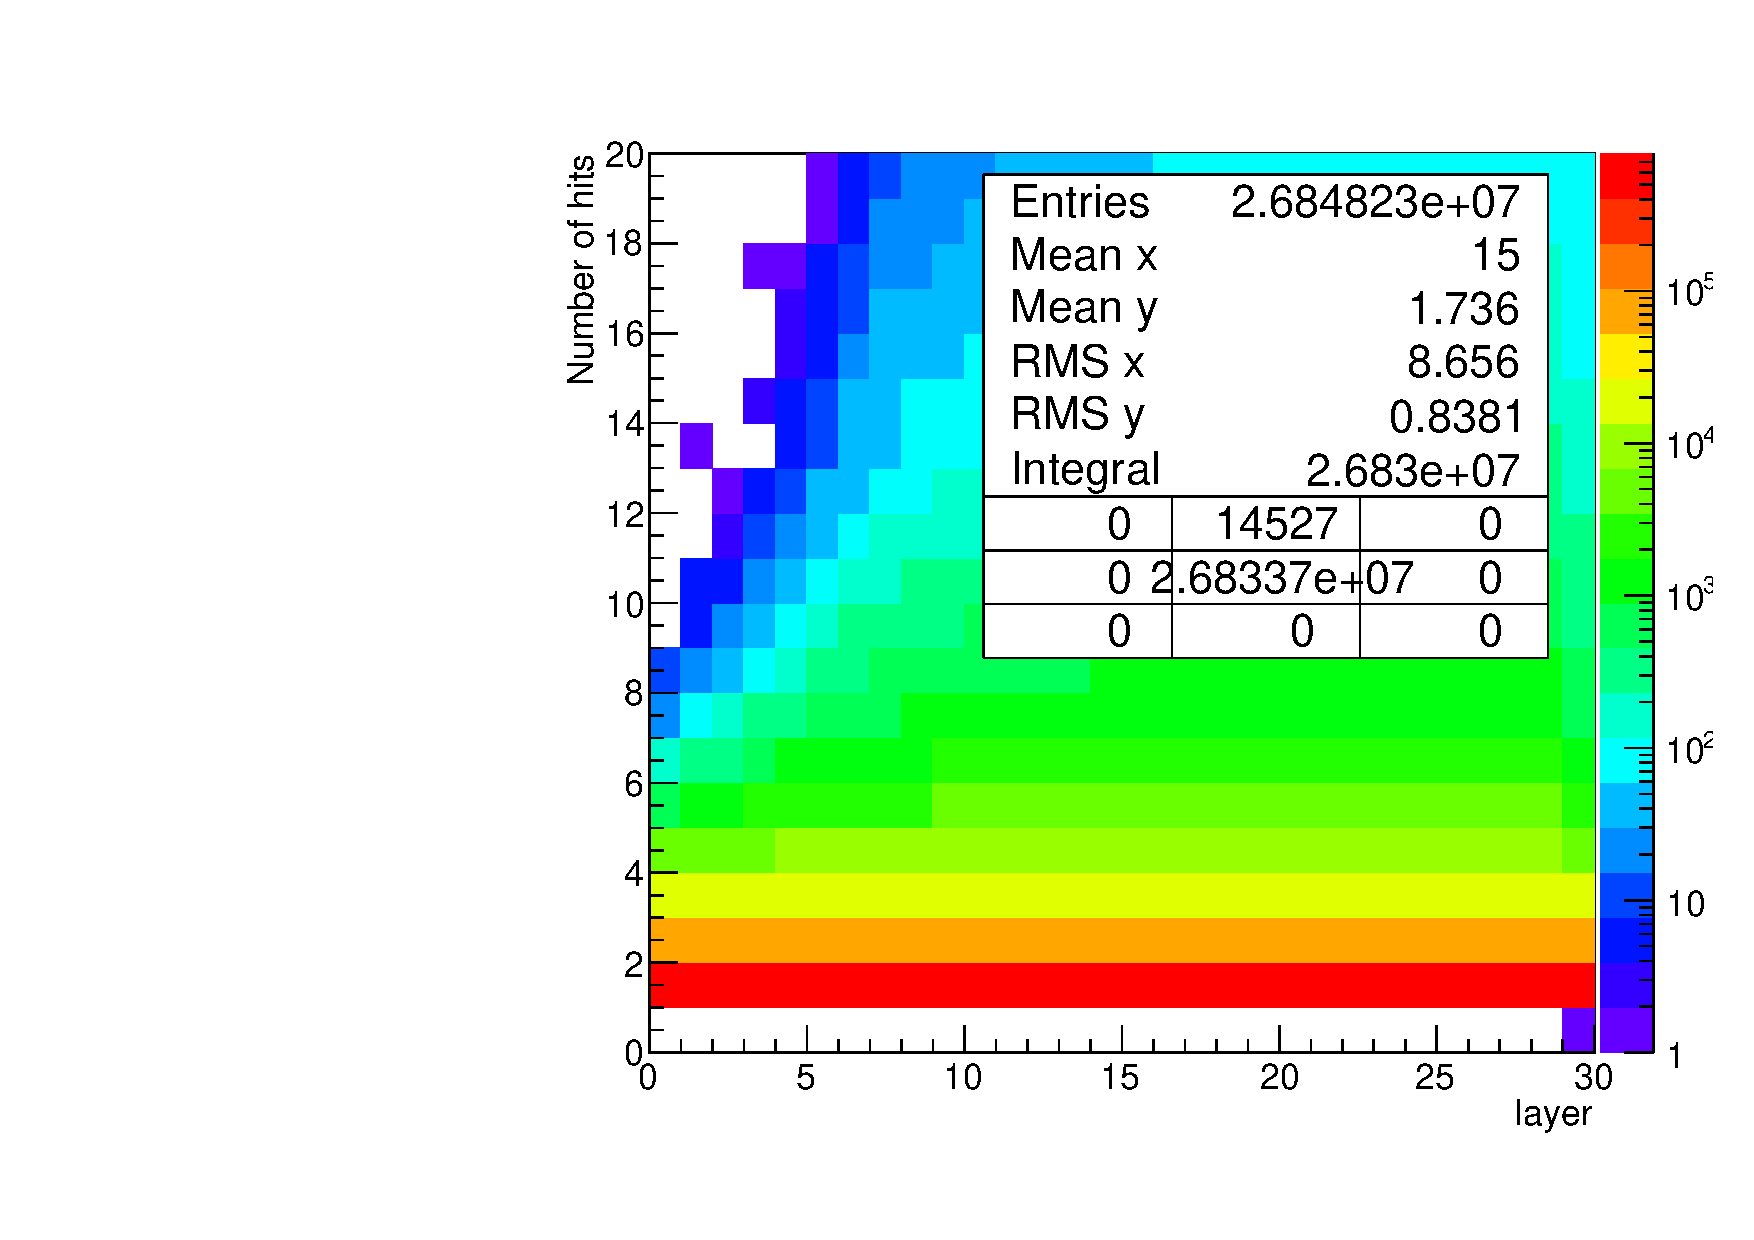
\includegraphics[width=\cmsFigWidth]{figures/mipHits.pdf}
    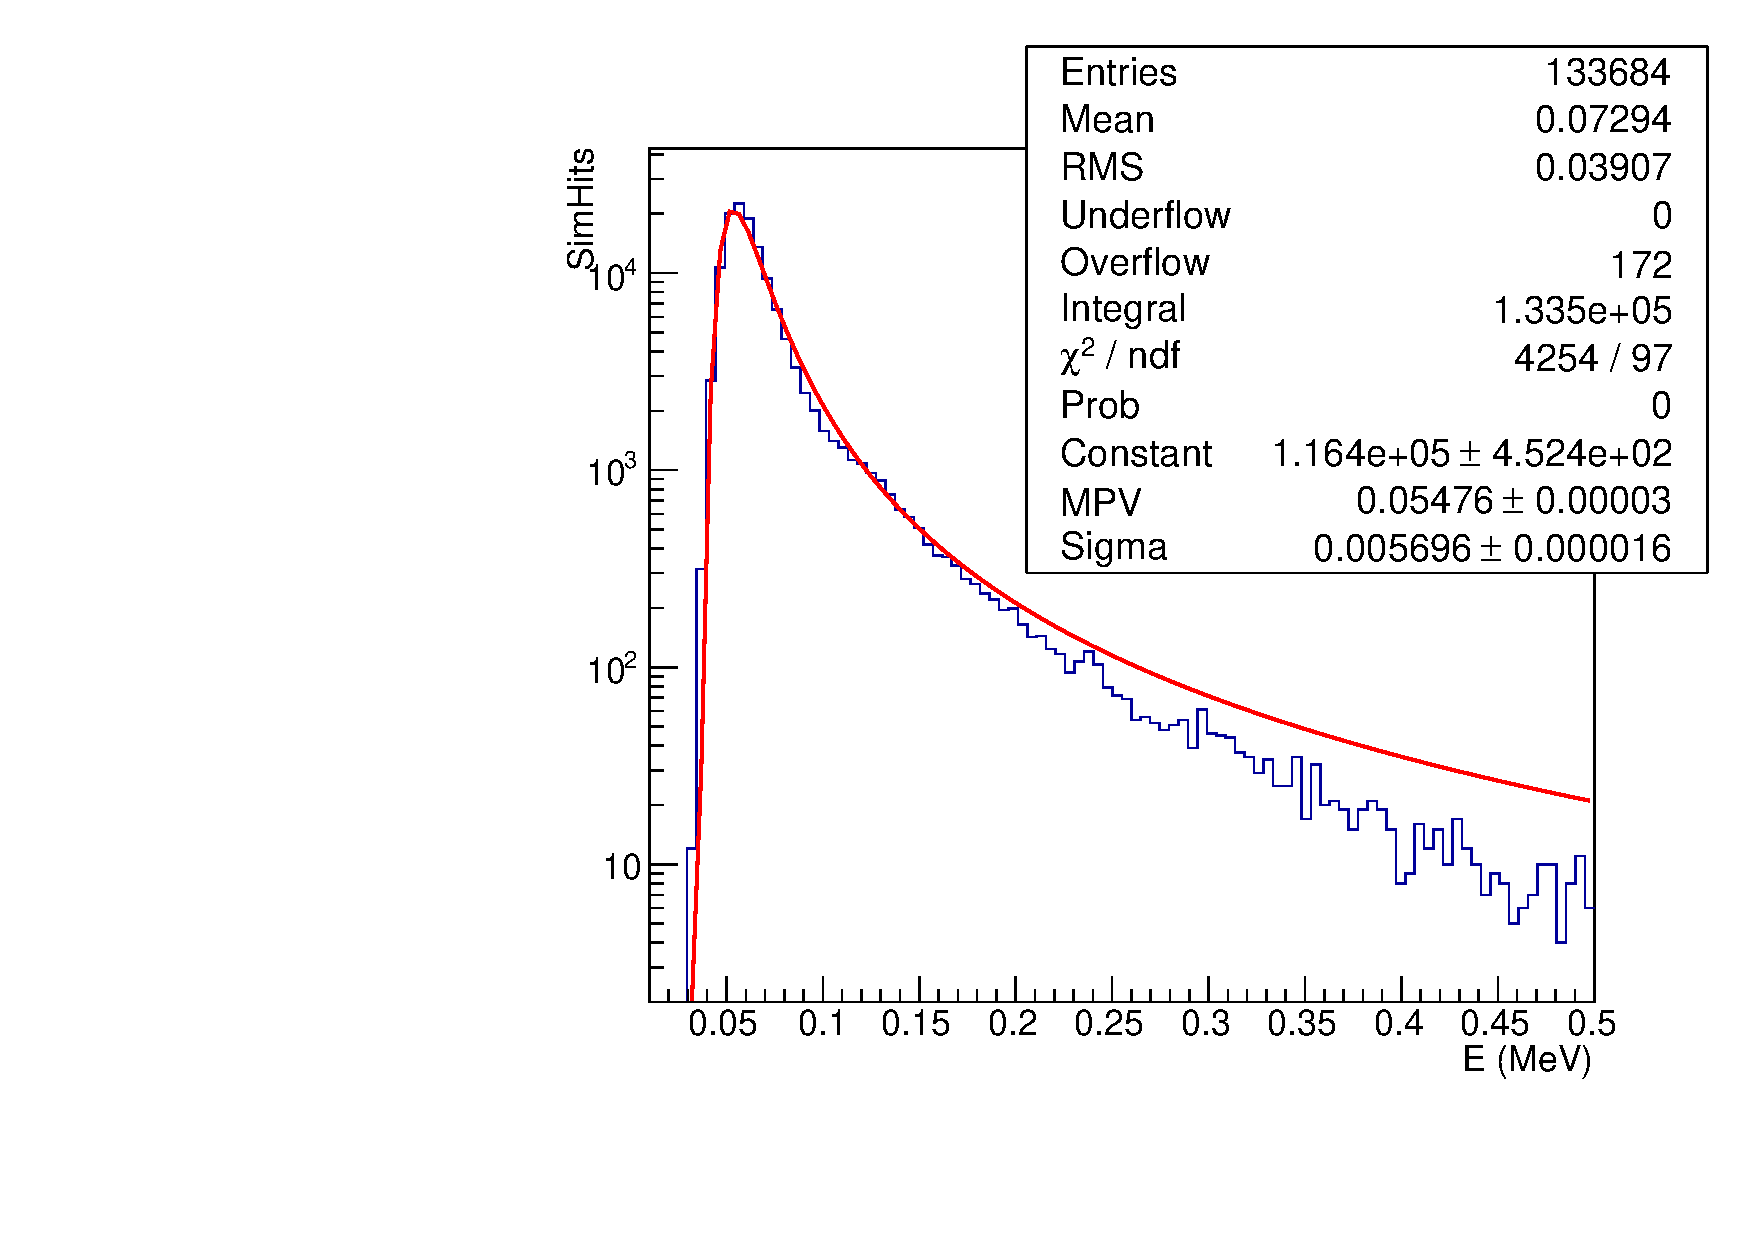
\includegraphics[width=\cmsFigWidth]{figures/mipDepositSel.pdf}
    \caption{}
    \label{fig:g4vis}
  \end{center}
\end{figure}


\subsection{Electronics calibration and noise}


